\textbf{{1. 5层结构的总结}}\\

OSI参考模型具有7层结构,而TCP/IP模型仅有4层结构(一般看作5层)。在OSI参考模型中表示层和会话层不是重点,大致浏览一遍即可,无须深究,所以只需掌握5层结构即可。读者应该能快速地默写出5层结构以及每层所完成的任务、功能、协议(遇到选择题能选对即可),5层参考模型各层的总结见表1-2。

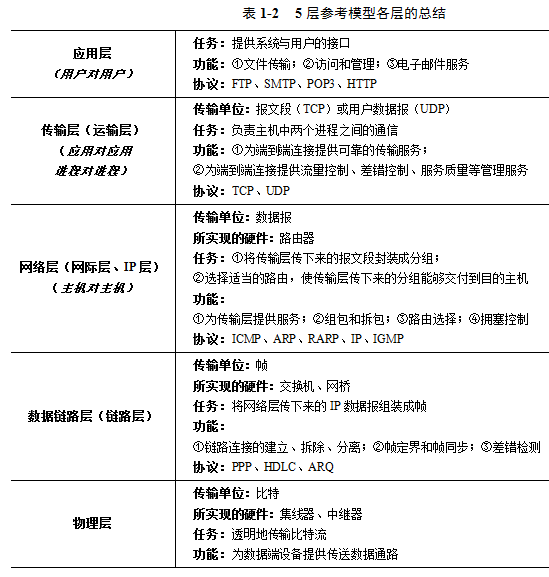
\includegraphics[width=3.12500in,height=3.28125in]{png-jpeg-pics/08D51F6D075F7F6763E3DA40367DB770.png}

\textbf{{2. OSI参考模型和TCP/IP模型的区别}}

{OSI参考模型和TCP/IP模型的特性对比见表1-3。}

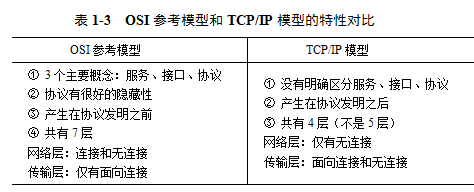
\includegraphics[width=3.59375in,height=1.45833in]{png-jpeg-pics/06F9DE75F91B172E6F21374CC3818251.png}

{\textbf{3. 会话层与表示层的基本功能}}

\textbf{{1.
会话层。}}{{会话层的主要功能是}\textbf{{在两个结点间建立、维护和释放面向用户的连接}}{,并对会话进行管理和控制,保证会话数据可靠传送。}}

\textbf{{2.
表示层。}}{{负责处理在两个内部数据表示结构不同的通信系统间交换信息的表示格式(数据格式转换,2013年统考真题考查了此功能),为}\textbf{{数据加密和解密}}{以及为提高传输效率提供必需的}\textbf{{数据压缩及解压}}{等功能。}}
